
	\section{Versuchsaufbau}
Um den Einfluss der Filtermodifikation zu untersuchen, wurden 3 Sensoren mit modifiziertem Print gefertigt. Die Printmodifikation betrifft die Eckfrequenz des Tiefpassfilters. Hierfür wurde je ein Print mit Eckfrequenz 70Hz, 100Hz sowie 500Hz gefertigt. Als Referenz wurde ein weiterer Sensor ohne Printmodifikation (Auslieferzustand Muster Sumitomo) gefertigt.\\
Die Sensoren wurden nicht abgeglichen, weshalb im Folgenden die Sensorwerte auf das jeweilige Maximum der Messungen normiert wurden.\\
Um messtechnisch den Einfluss der Filtermodifikation zu validieren, wurden jeweils ein Sensor mit Modifikation (Device under Test, DuT) sowie der nicht-modifizierte Sensor  ``Rücken an Rücken'' gestellt. Während der Messung wurde das Nullpunktsignal für einige Sekunden aufgezeichnet, wobei die Sensoren auf einem Tisch liegen gelassen wurden. Anschliessend wurden die Sensoren jeweils Steckerseitig aneinandergepresst, womit beide Sensoren (DuT und Referenz) jeweils etwa die gleiche Dehnung erfahren sollten. 
	\begin{figure}[H]
		\centering
		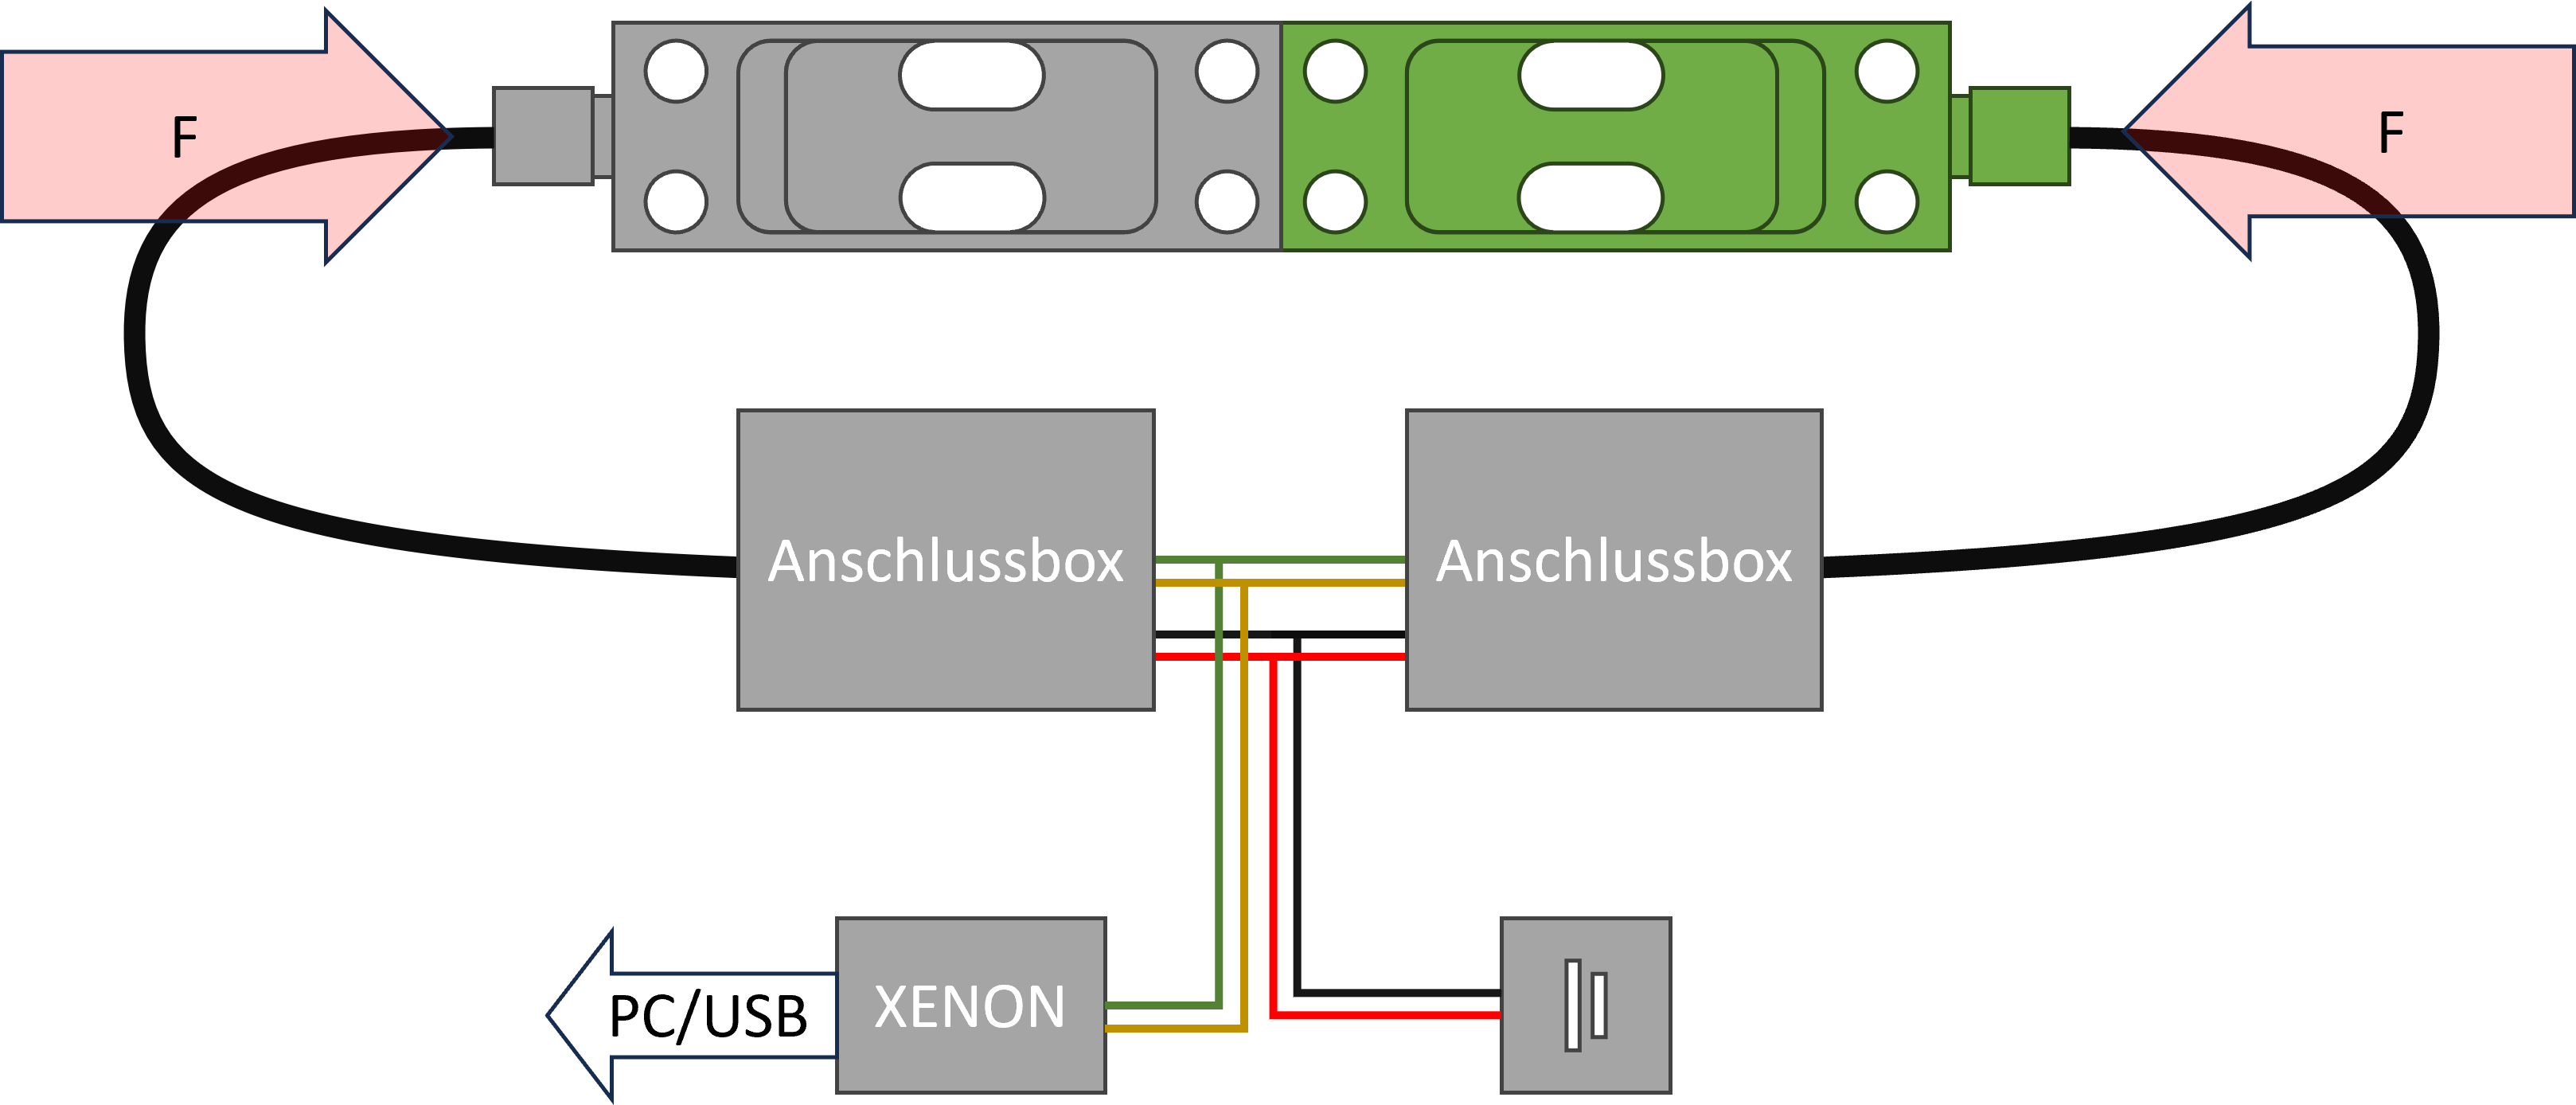
\includegraphics[width=1\linewidth]{Aufbau}
		\caption{Versuchsaufbau; grün: DuT, grau: Referenz}
		\label{fig:screenshot001}
	\end{figure}
\noindent Die Sensoren wurden mit einem Labornetzteil mit 24 V gespiesen, zur Datenerfassung wurde das USB-Interface mit XENON eingesetzt. Die Parameter sind in Tabelle \ref{tab:params} aufgelistet. Der Referenz-Sensor ist für alle Messungen auf CH0, das DuT auf CH1.
	\begin{table}[H]
		\centering
		\caption{Messparameter}
	\begin{tabular}{l|l}
		Abtastfrequenz & 2000 Hz \\
		\hline
		Speisung & 24 V \\
		\hline
		Messdauer & $\sim$ 60 s \\
	\end{tabular}	
	\label{tab:params}
	\end{table}
\begin{table}[H]
	\centering
	\caption{Getestete DuTs}
	\begin{tabular}{c|c}
		\textbf{\#DuT} &\textbf{ Eckfrequenz $f_c$ [Hz]}\\
		\hline
		DuT 1 & 70 \\
		DuT 2 & 100\\
		DuT 3 & 500\\
	\end{tabular}	
	\label{tab:params}
\end{table}
	\section{Resultate \& Diskussion}
	\subsection{Modifikation 70 Hz}
Abbildung \ref{fig:refsolo} zeigt den Signalverlauf des Referenzsensors. Das DuT und die Referenz wurden zu erst zweimal schlagartig  und anschliessend rampenartig belastet. Die schlagartige Belastung resultiert in ''Spikes``, welche unmittelbar zu Beginn des Signalanstiegs zu erkennen sind.
	\begin{figure}[H]
		\centering
		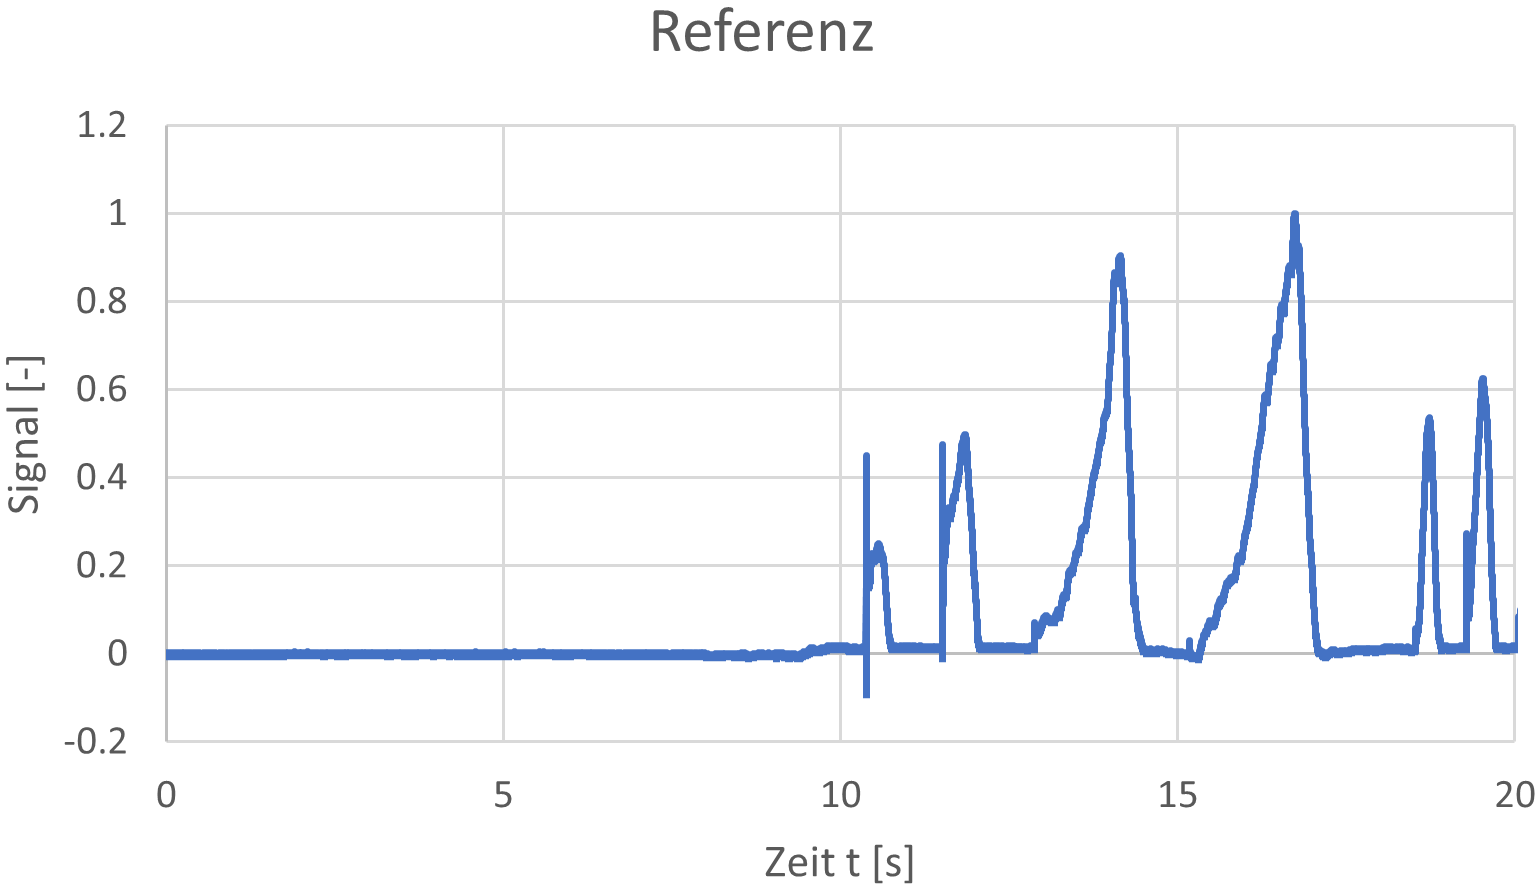
\includegraphics[width=1\linewidth]{img_70Hz/ref_solo}
		\caption{Signalverlauf Referenzsensor}
		\label{fig:refsolo}
	\end{figure}
\noindent Die Abbildung \ref{fig:dutsolo} zeigt den zu Abbildung \ref{fig:refsolo} simultanen Signalverlauf des DuT. Aufgrund des modifizierten Filters sind hier keine Spikes auszumachen. 
	\begin{figure}[H]
		\centering
		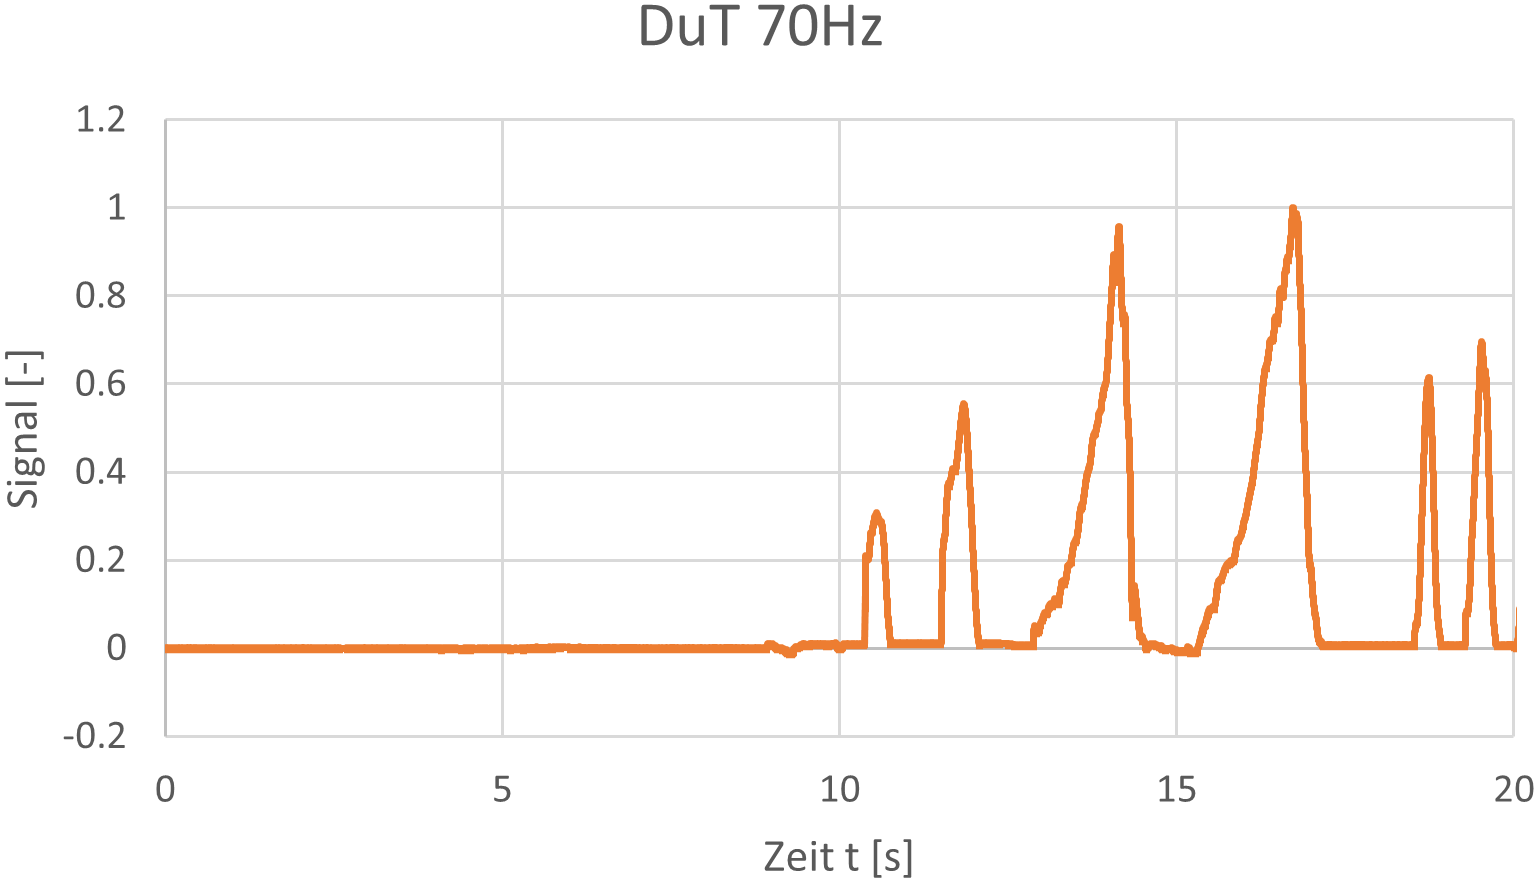
\includegraphics[width=1\linewidth]{img_70Hz/dut_solo}
		\caption{Signalverlauf DuT}
		\label{fig:dutsolo}
	\end{figure}
	\begin{figure}[H]
		\centering
		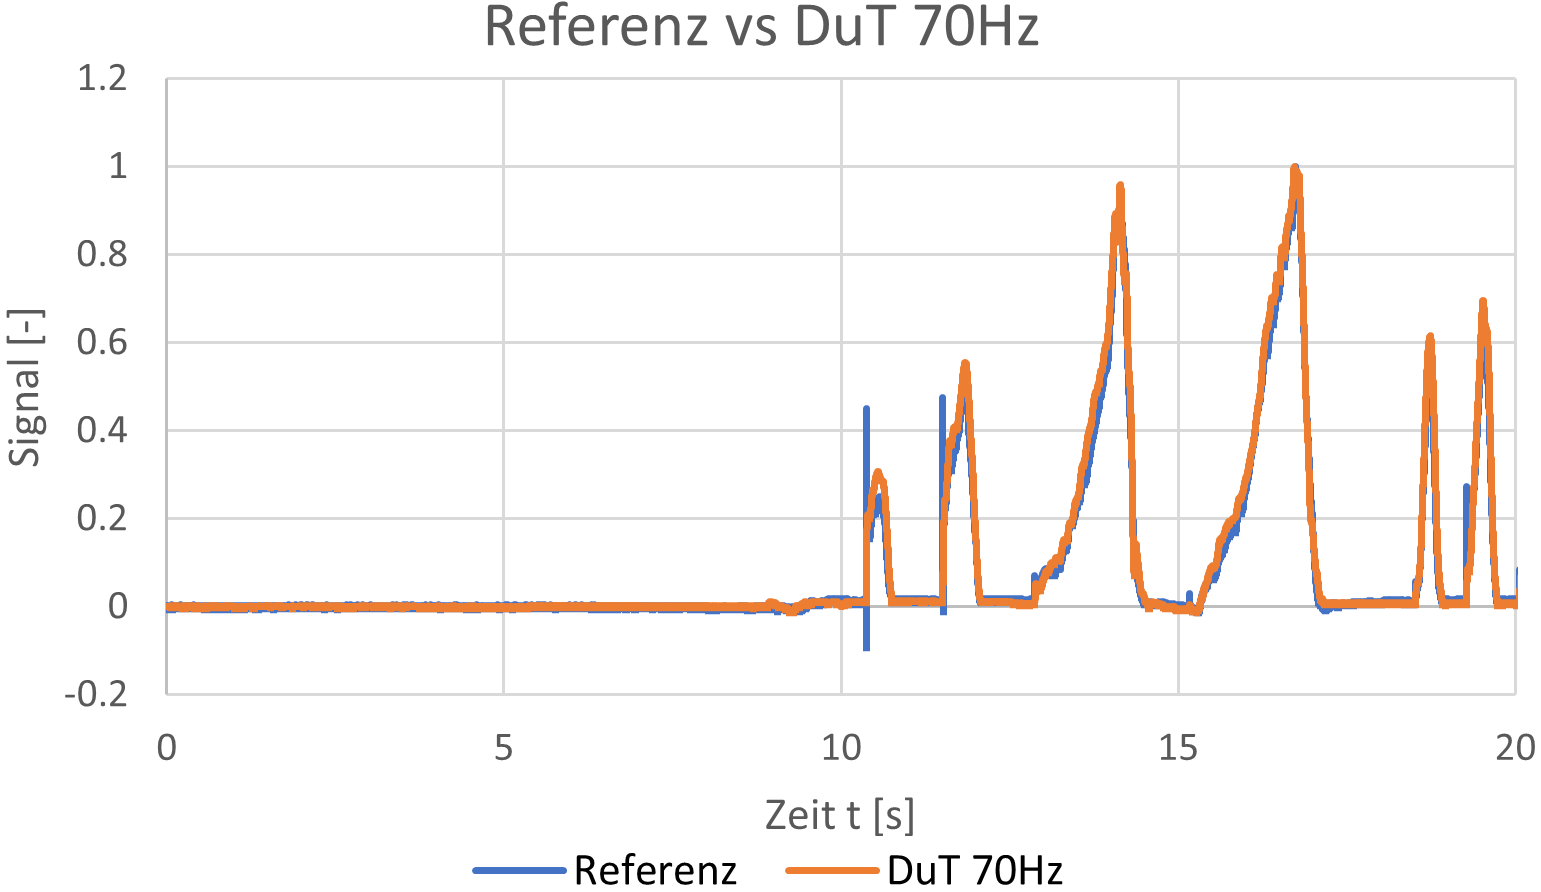
\includegraphics[width=1\linewidth]{img_70Hz/comp_total}
		\caption{Vergleich Referenz und DuT}
		\label{fig:comptotal}
	\end{figure}
\noindent Die Abbildung \ref{fig:compdetail} zeigt weiter, dass der Signalverlauf des DuT insgesamt glatter ist als jener der Referenz.
	\begin{figure}[H]
		\centering
		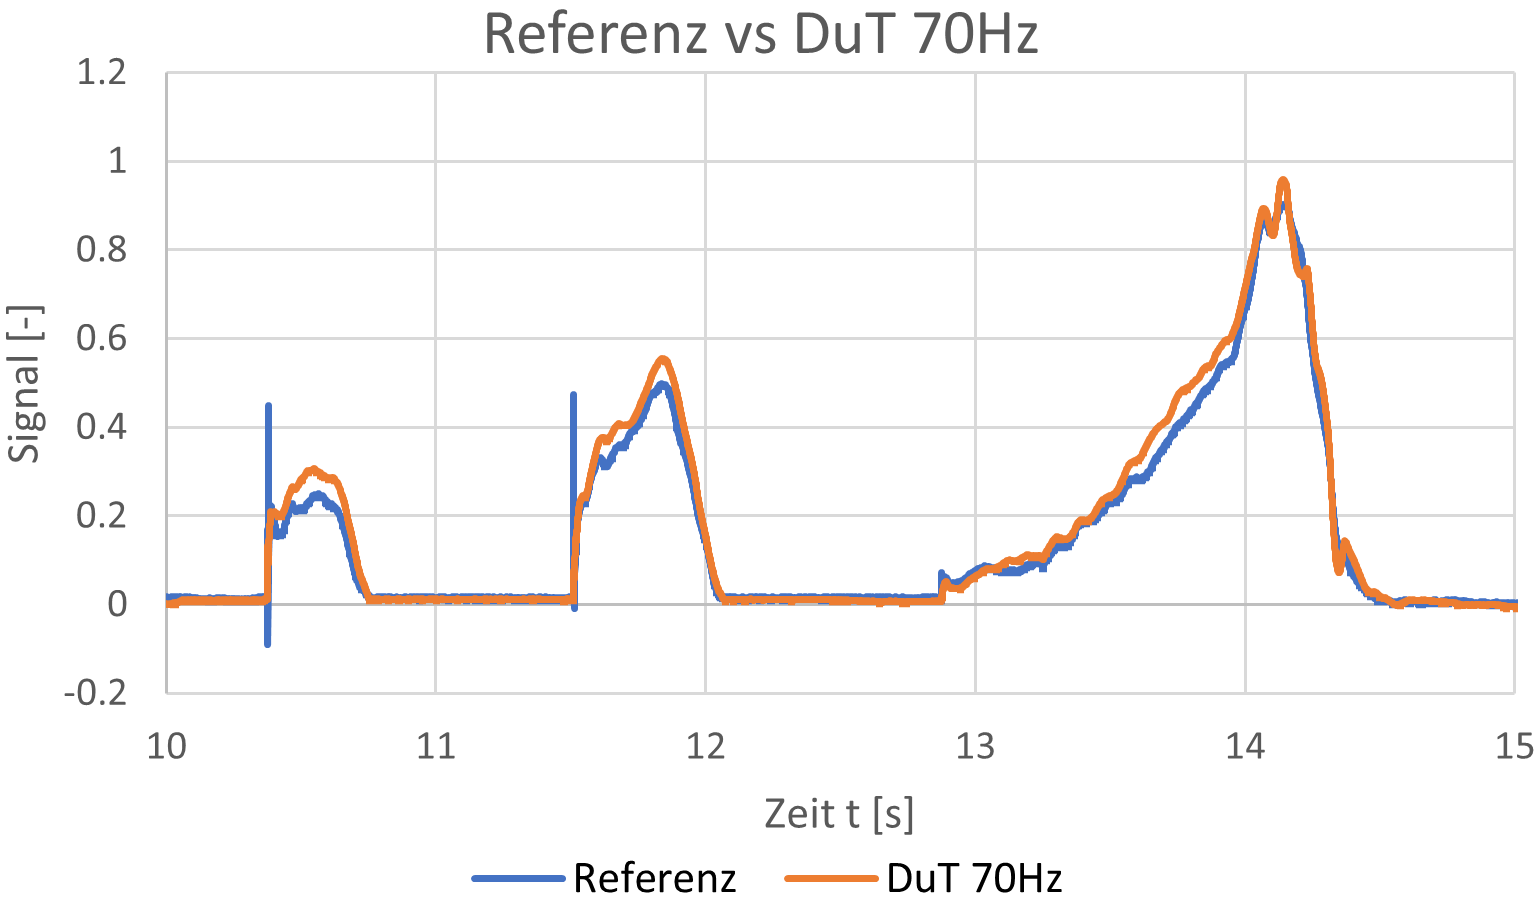
\includegraphics[width=1\linewidth]{./img_70Hz/comp_detail}
		\caption{Ausschnitt aus Vergleich (Abbildung \ref{fig:comptotal})}
		\label{fig:compdetail}
	\end{figure}
\noindent Das Band des Rauschens auf dem Ruhesignal fällt beim DuT wesentlich schmaler aus als bei der Referenz wie in Abbildung \ref{fig:compnp} zu erkennen ist.
	\begin{figure}[H]
		\centering
		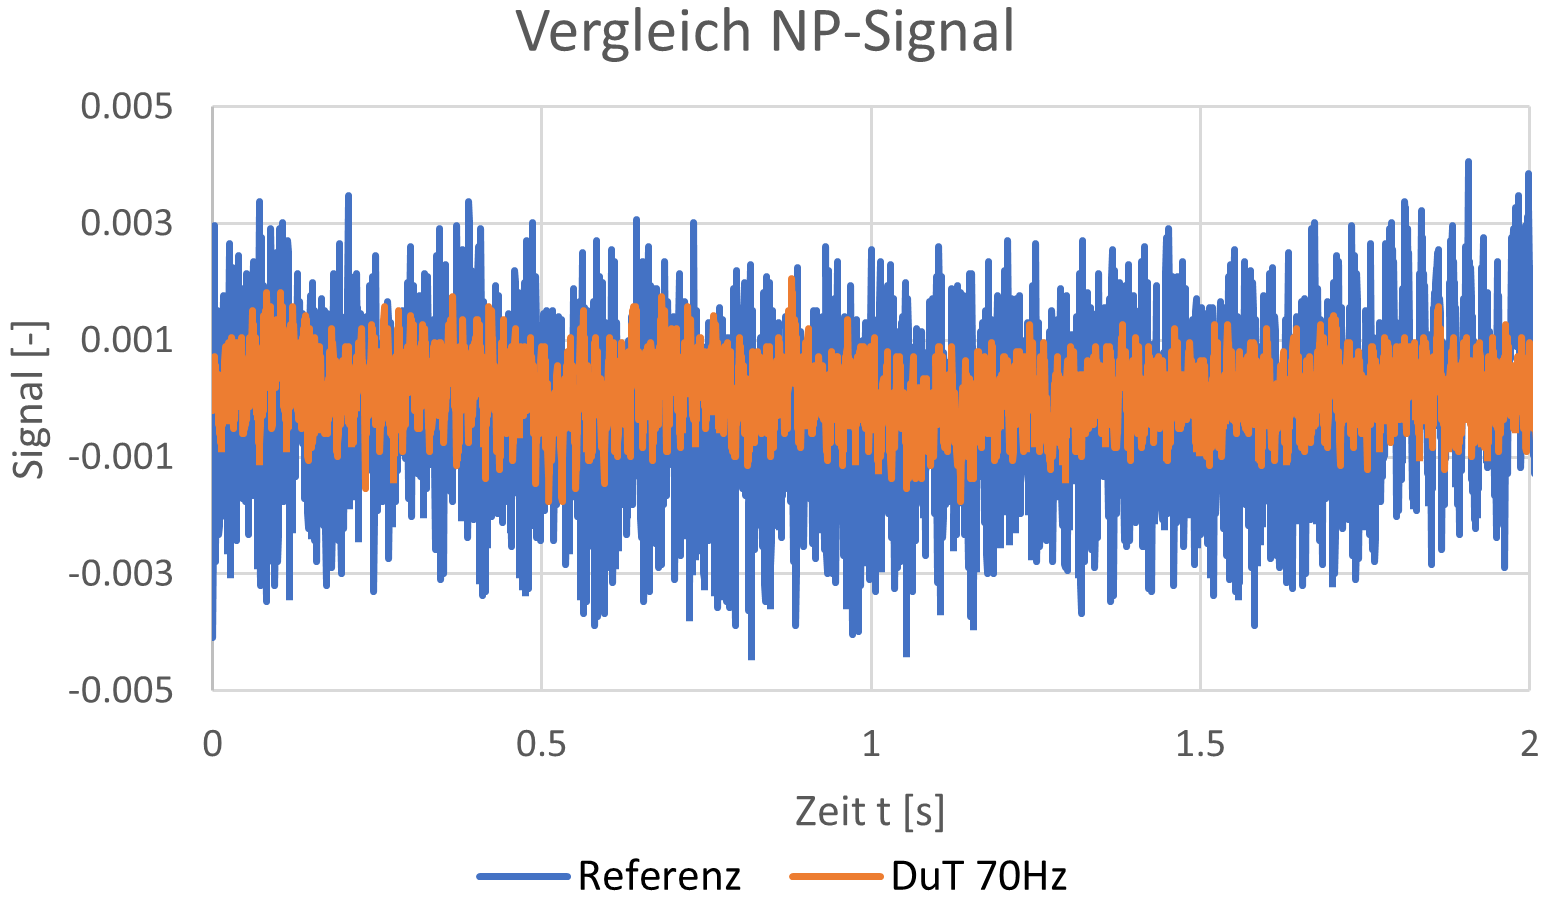
\includegraphics[width=1\linewidth]{img_70Hz/comp_NP}
		\caption{Vergleich des Nullpunktsignals (DuT und Referenz in Ruhe auf einer Tischfläche liegend)}
		\label{fig:compnp}
	\end{figure}
\noindent Die Fourieranalyse bestätigt vorherige Resultate punkto Rauschverhalten. Im Spektrum des DuT-Signals werden höhere Frequenzen deutlich gedämpft. Es fällt jedoch auf, dass rund alle 250Hz markante Spikes vorhanden sind.
	\begin{figure}[H]
		\centering
		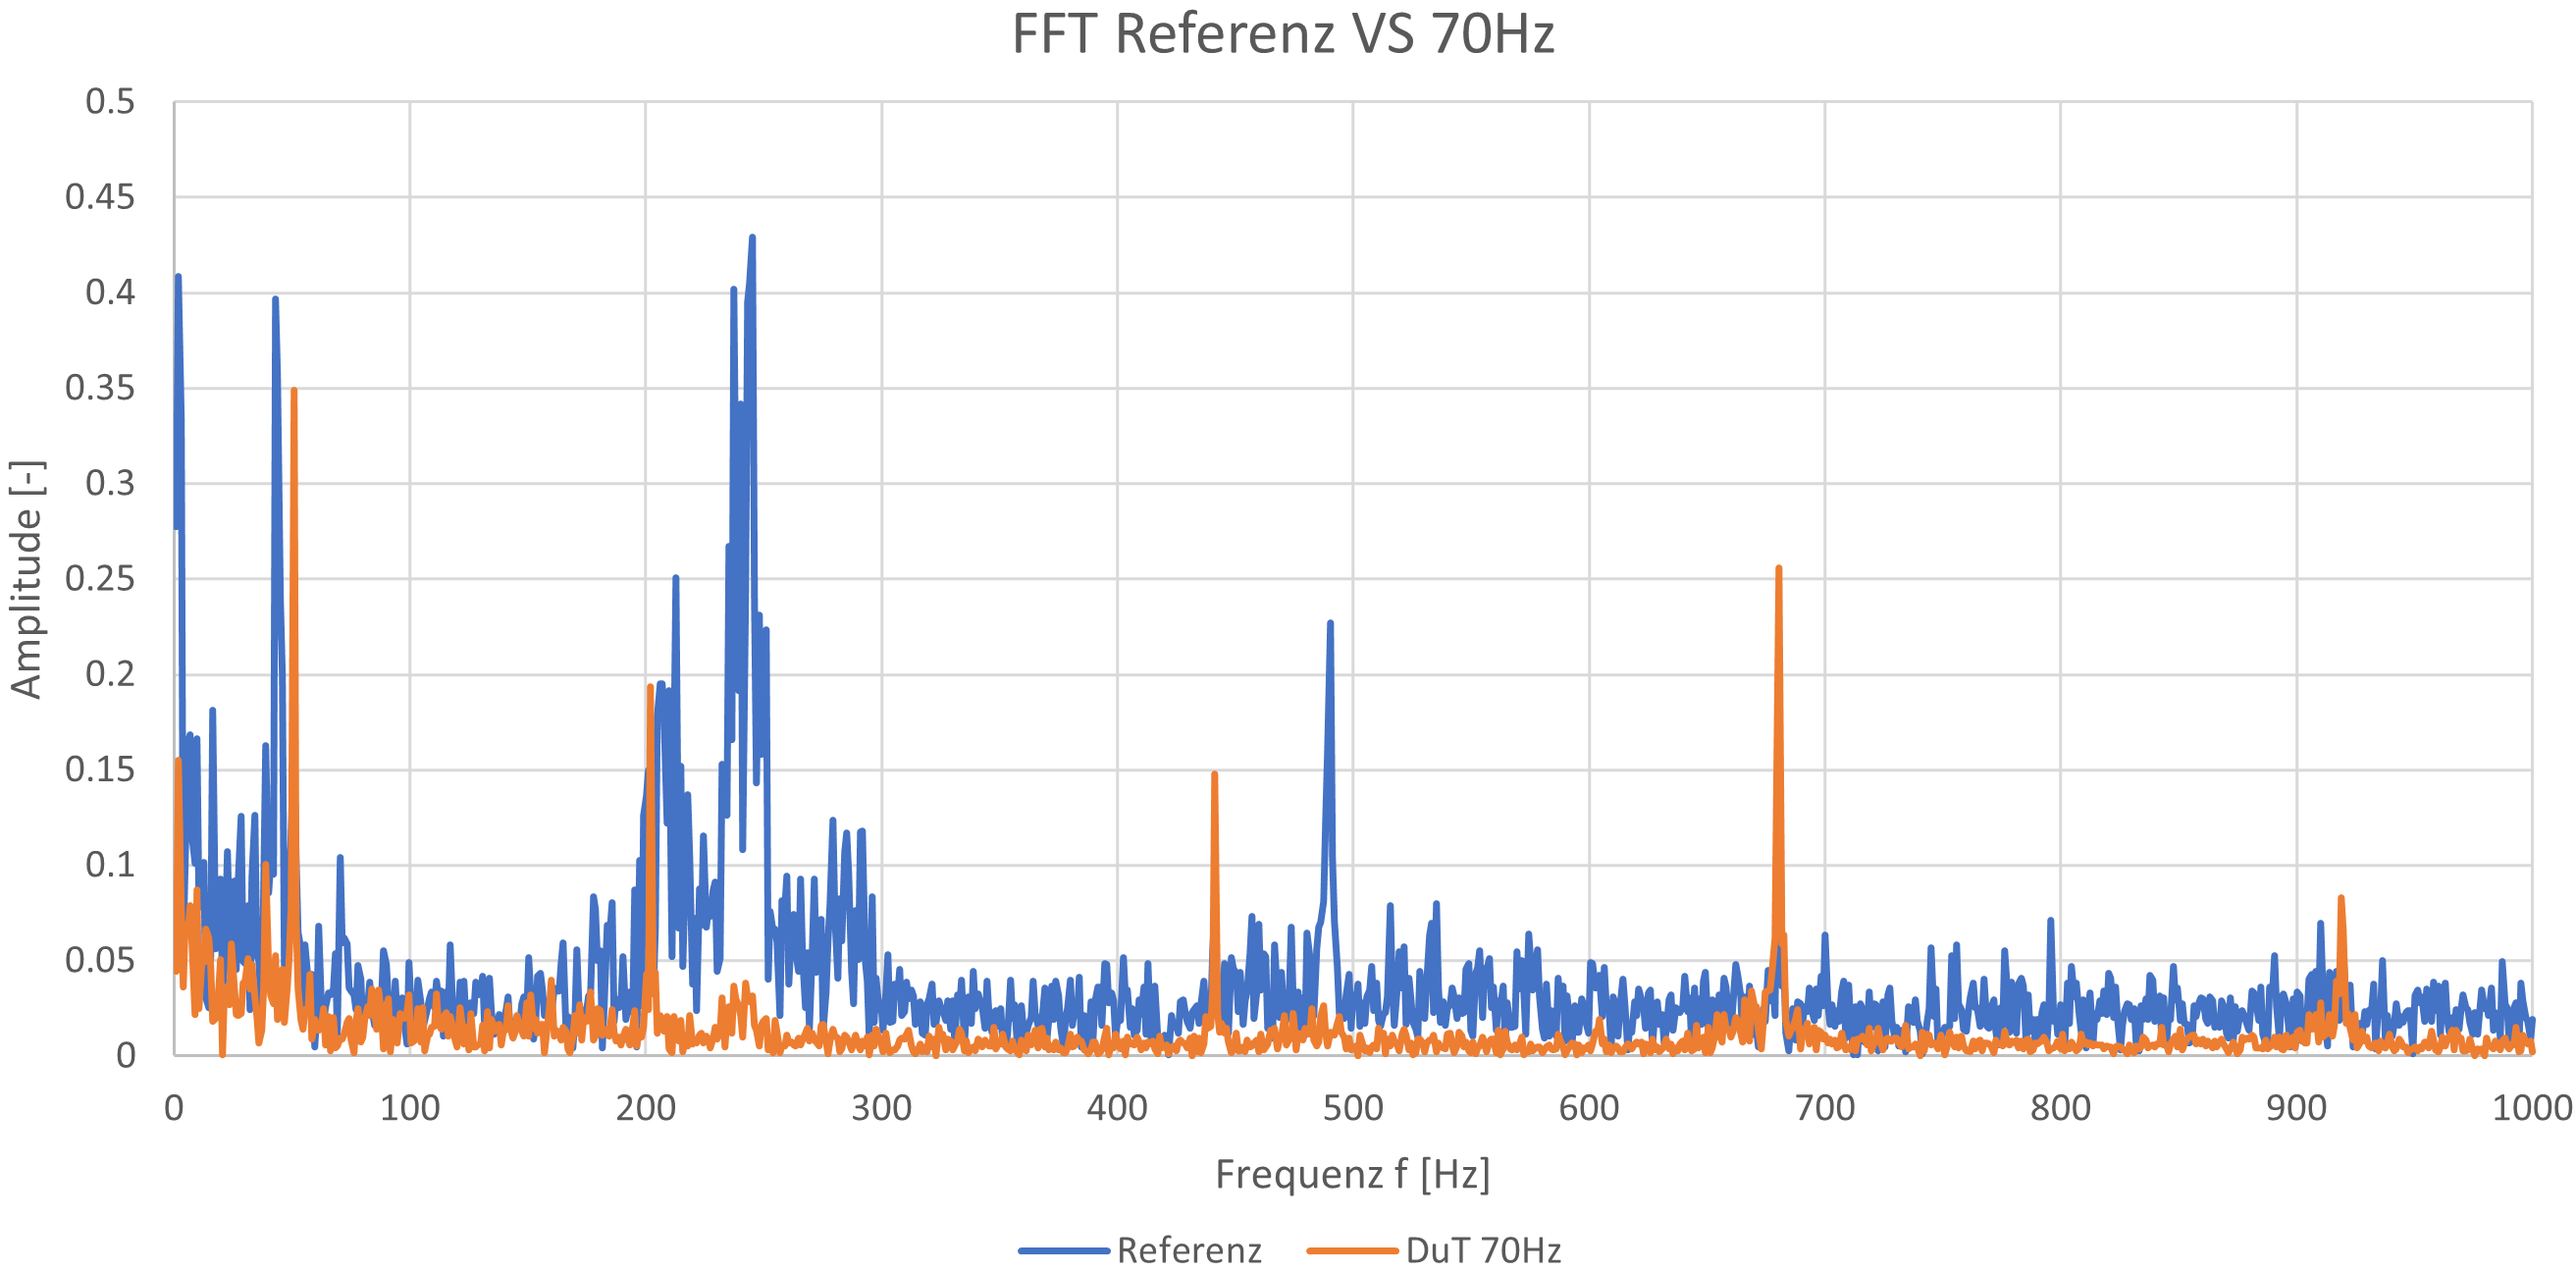
\includegraphics[width=1\linewidth]{img_70Hz/comp_FFT}
		\caption{(Fast) Fouriertransformation der Nullpunktsignale}
		\label{fig:compfft}
	\end{figure}
	
	\subsection{Modifikation 100 Hz}
Mit dem zweiten DuT (100Hz) wurden obige Messungen weitestgehend wiederholt. Da die Last / Dehnung nicht automatisiert aufgebracht werden konnte, sieht der Signalverlauf etwas anders aus. Es wurde wieder zu erst einige Sekunden Nullpunktsignal gefolgt von zwei schlagartigen und anschliessend weiteren rampenartigen Belastungen aufgezeichnet. Der Verlauf des Referenzsignals ist der Abbildung \ref{fig:screenshot002} zu entnehmen. Auch hier sind die schlagartigen Belastungen an den Spikes zu erkennen.
	\begin{figure}[H]
		\centering
		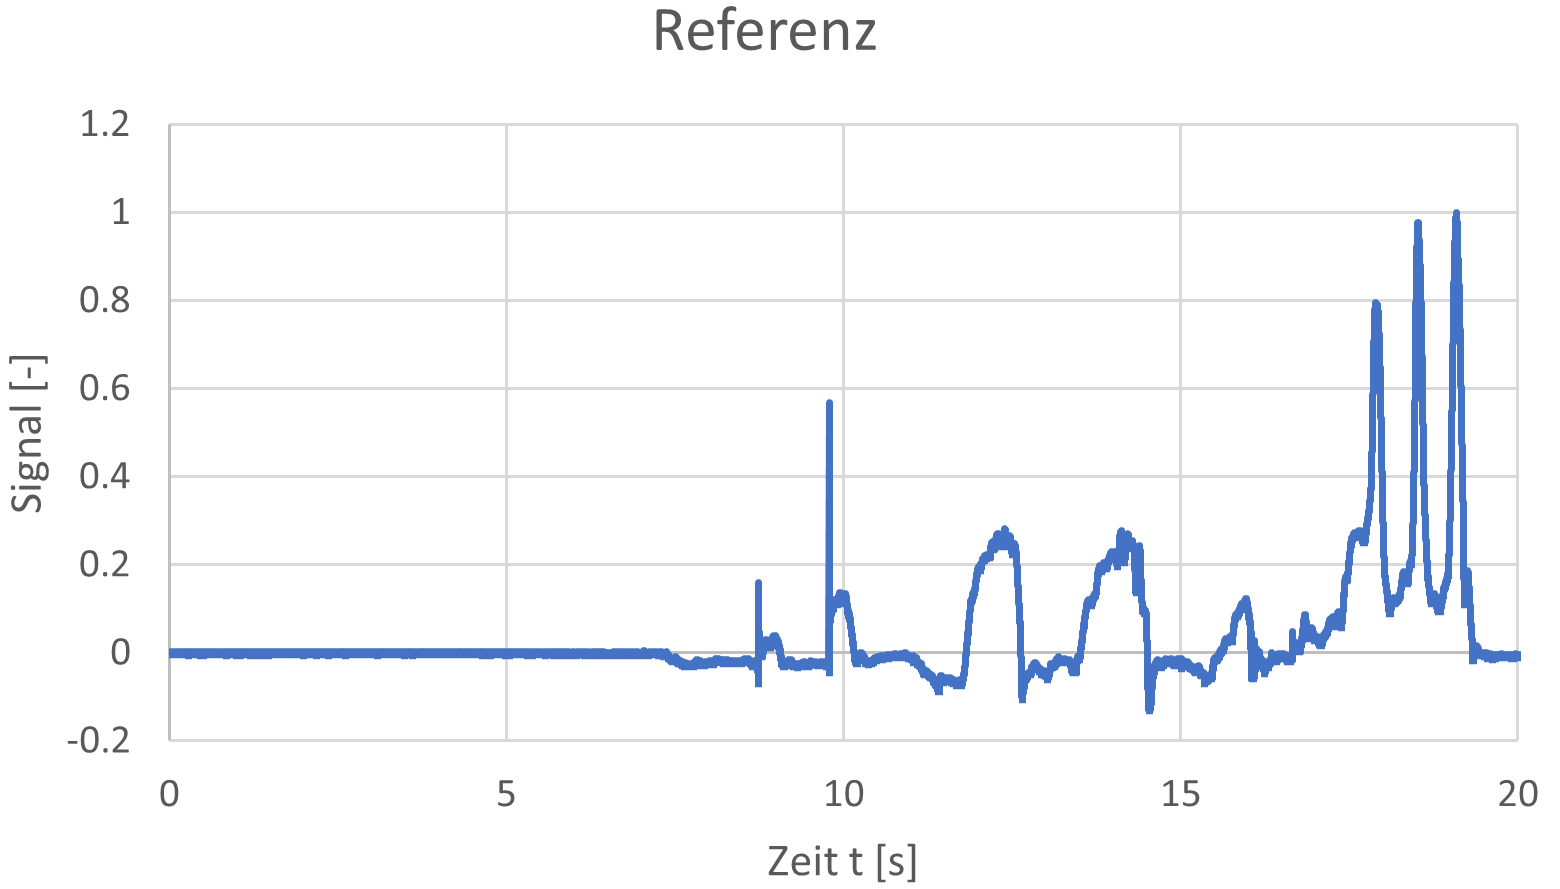
\includegraphics[width=1\linewidth]{Ref_solo_100Hz}
			\caption{Signalverlauf Referenzsensor}
		\label{fig:screenshot002}
	\end{figure}
\noindent Wie bereits bei der Modifikation mit Eckfrequenz 70Hz filtert auch das DuT mit Eckfrequenz 100Hz die Spikes mehrheitlich heraus, wie in der untenstehenden Abbildung \ref{fig:dutOnly100} zu erkennen ist.
	\begin{figure}[H]
		\centering
		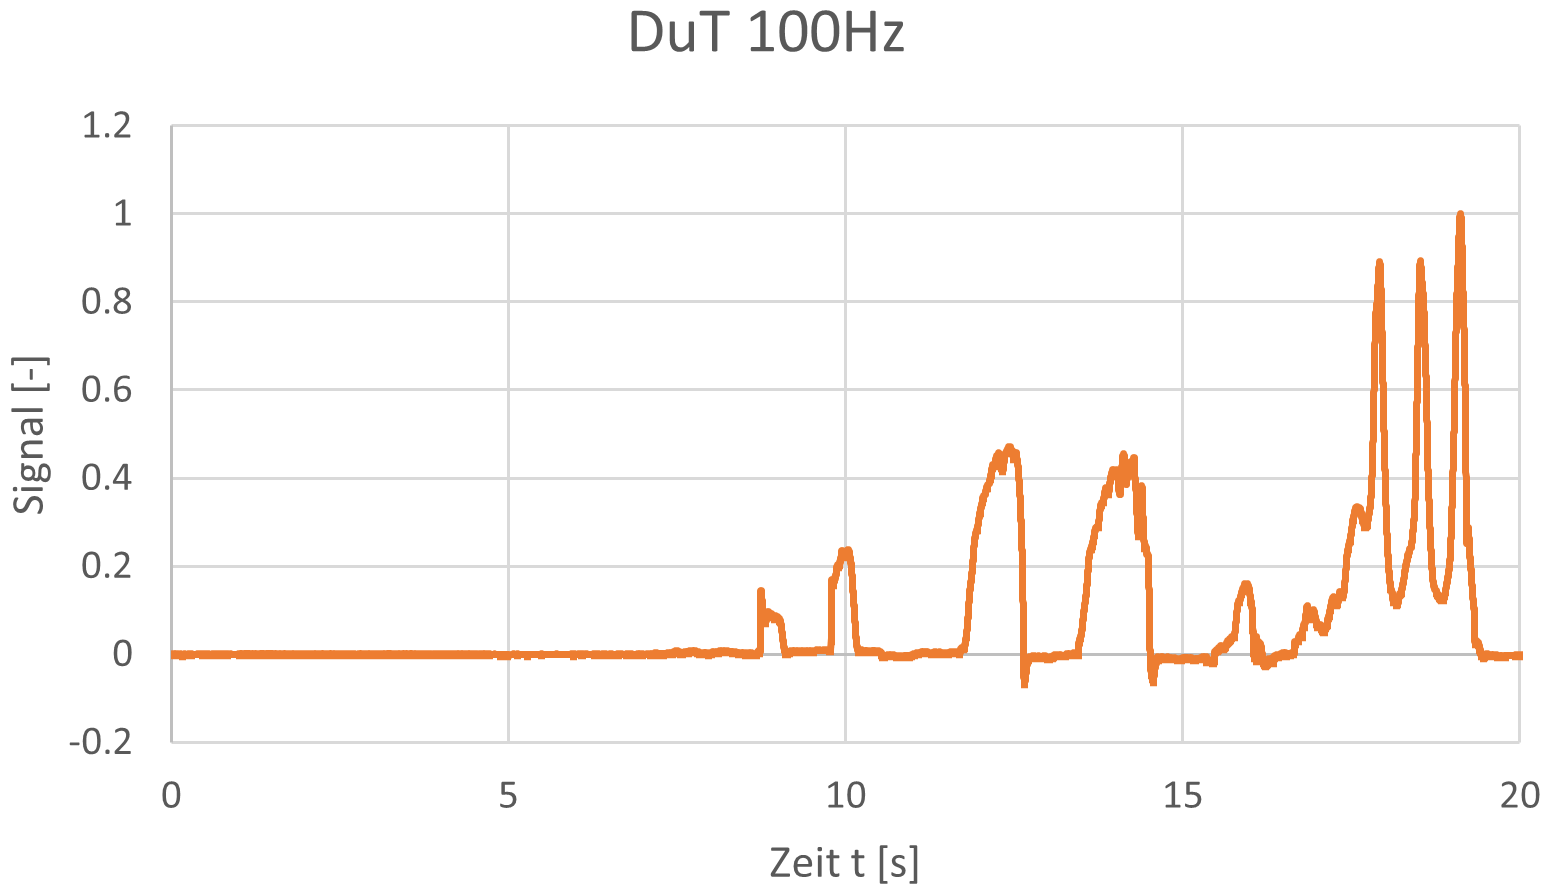
\includegraphics[width=1\linewidth]{Dut_solo_100Hz}
		\caption{Signalverlauf DuT}
		\label{fig:dutOnly100}
	\end{figure}
\noindent Die beiden Signalverläufe sind in Abbildung \ref{fig:partcomp100hz} überlagert. Hier fällt auf, dass die Referenz ein inkonsistentes Nullpunkverhalten aufweist. 
	\begin{figure}[H]
		\centering
		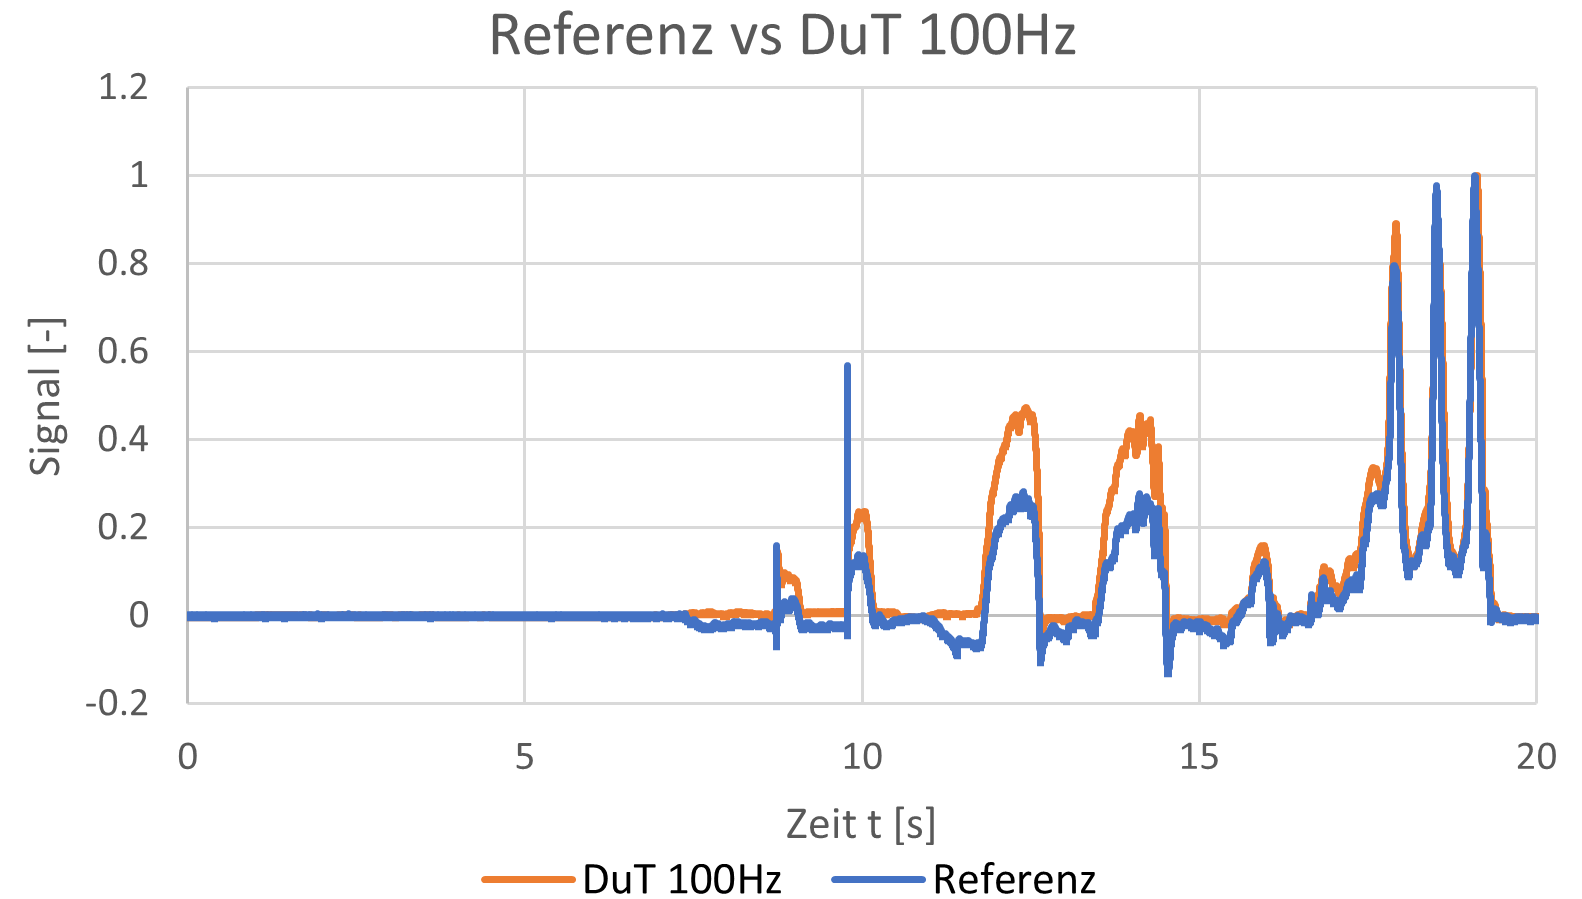
\includegraphics[width=1\linewidth]{part_comp_100Hz}
		\caption{Vergleich Referenz und DuT}
		\label{fig:partcomp100hz}
	\end{figure}
\noindent Um die Unterschiede zwischen DuT und Referenz hervorzuheben, ist in der Abbildung \ref{fig:comp100hz} ein Ausschnitt aus obigem Diagramm zu sehen. Der Ausschnitt zeigt nochmal die Dämpfung der Spikes sowie das inkonsistente ''Return to zero``-Verhalten der Referenz. Weiter kann am Wellenverlauf bei anhaltender Belastung erkannt werden, dass das DuT (orange) einen glatteren Signalverlauf aufweist.
	\begin{figure}[H]
		\centering
		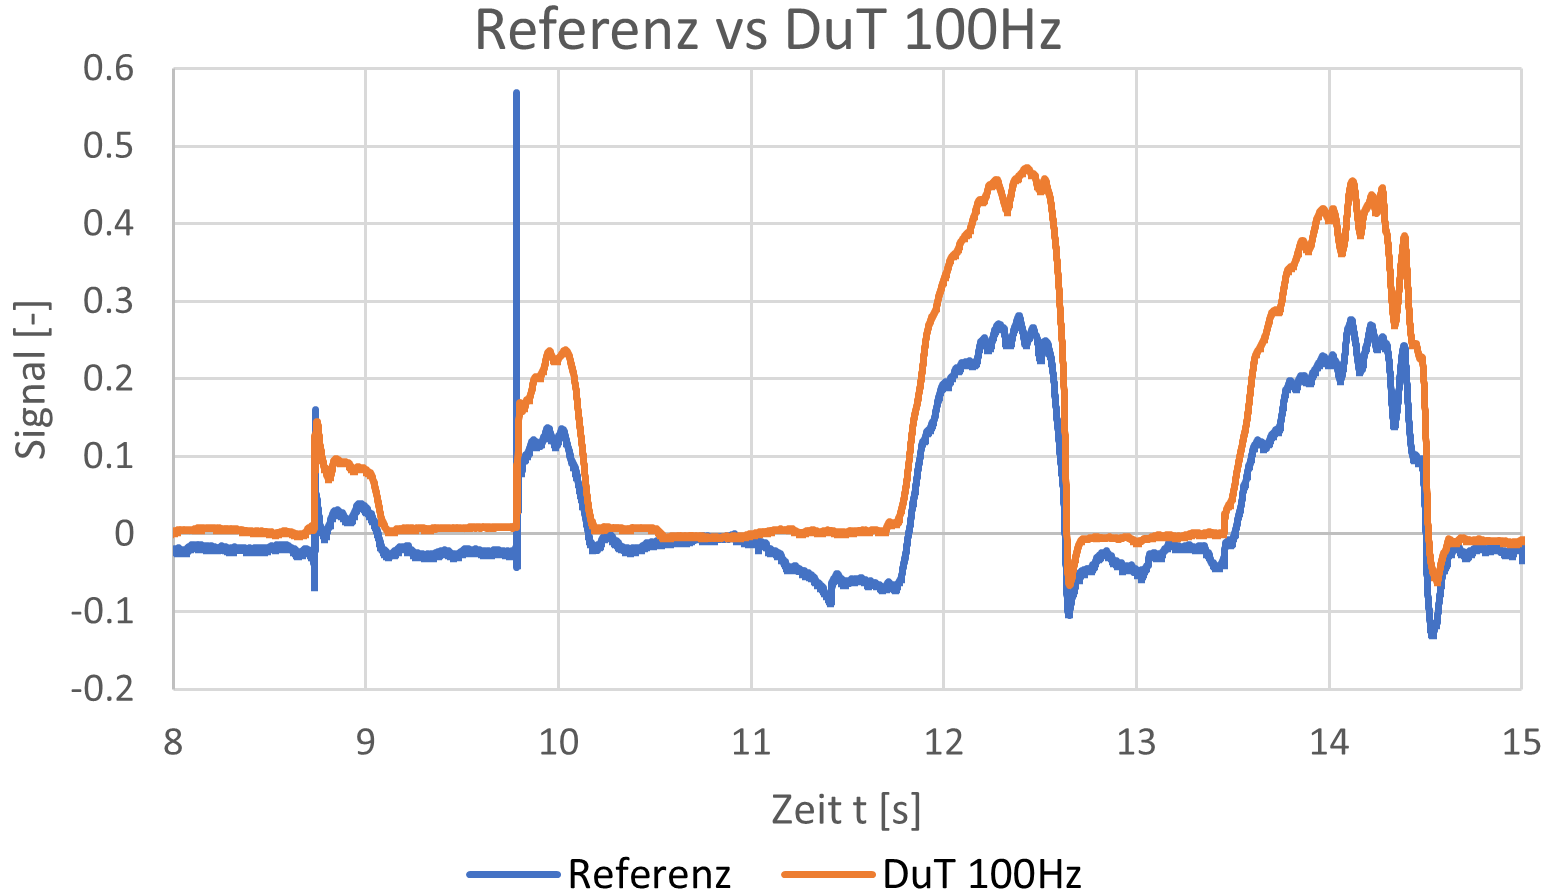
\includegraphics[width=1\linewidth]{comp_100Hz}
		\caption{Ausschnitt aus Vergleich (Abbildung \ref{fig:partcomp100hz})}
		\label{fig:comp100hz}
	\end{figure}
\noindent Wie bereits beim DuT mit $f_c=70$Hz ist auch beim DuT mit  $f_c=100$Hz eine klare Rauschminimierung beim Nullpunktsignal auszumachen.
	\begin{figure}[H]
		\centering
		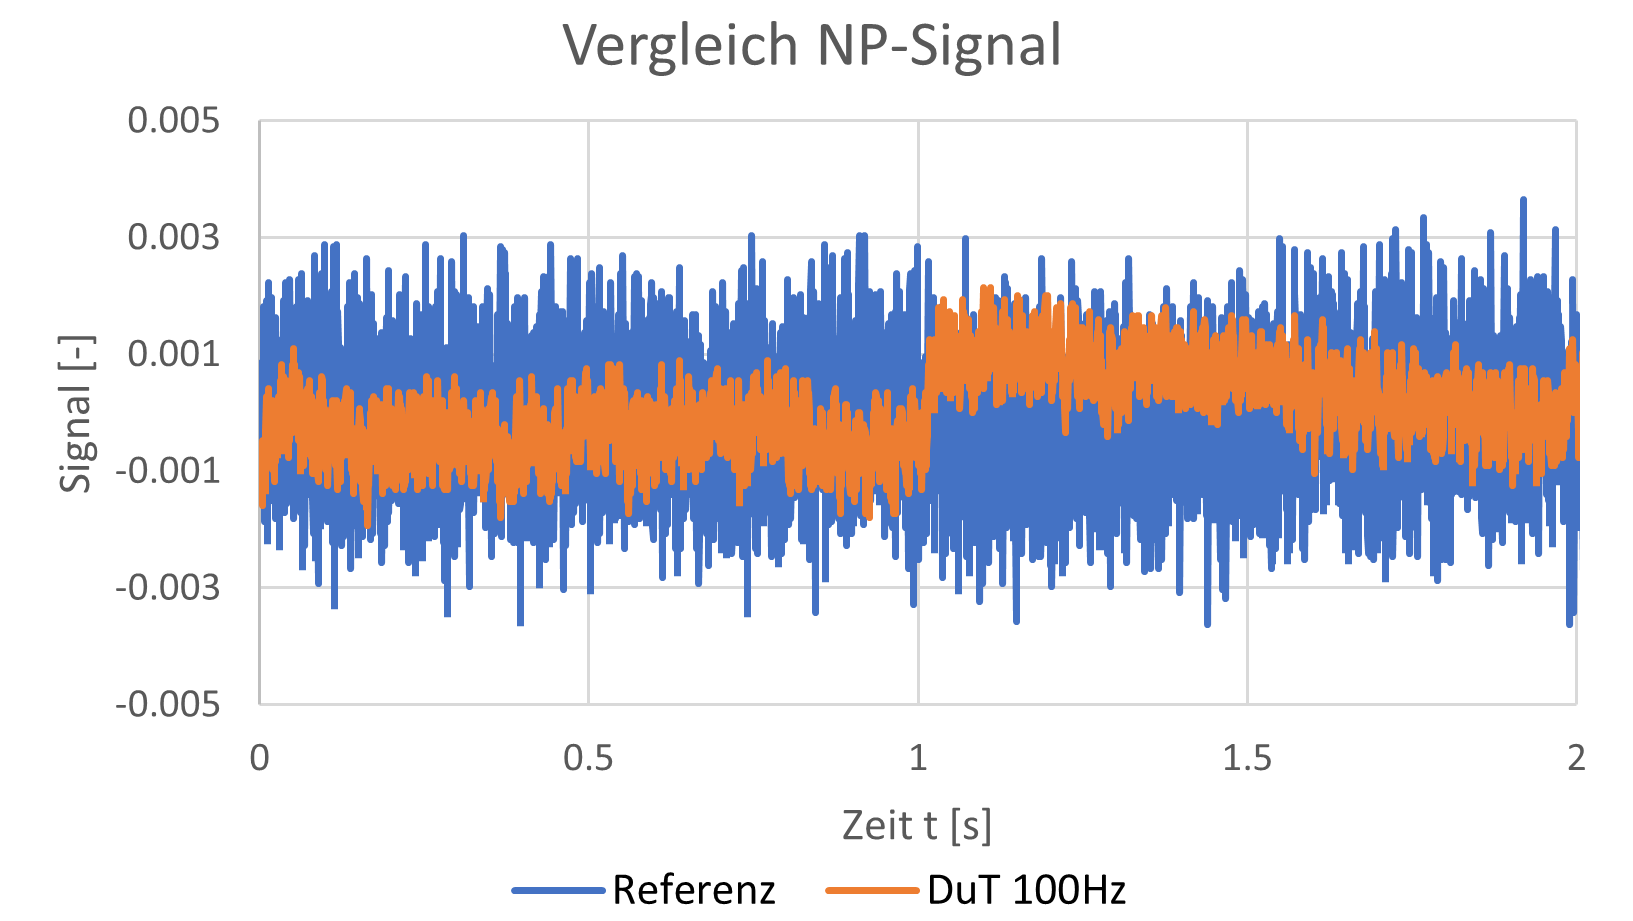
\includegraphics[width=1\linewidth]{Np_comp_100Hz}
		\caption{Vergleich des Nullpunktsignals (DuT und Referenz in Ruhe auf einer Tischfläche liegend)}
		\label{fig:npcomp100hz}
	\end{figure}
\noindent Die Fourieranalyse bestätig auch hier die Wirksamkeit des Filters. Wie bereits beim ersten DuT sind auch hier einige periodische Spikes ab 400Hz mit einem Abstand von rund 80Hz auszumachen.
	\begin{figure}[H]
		\centering
		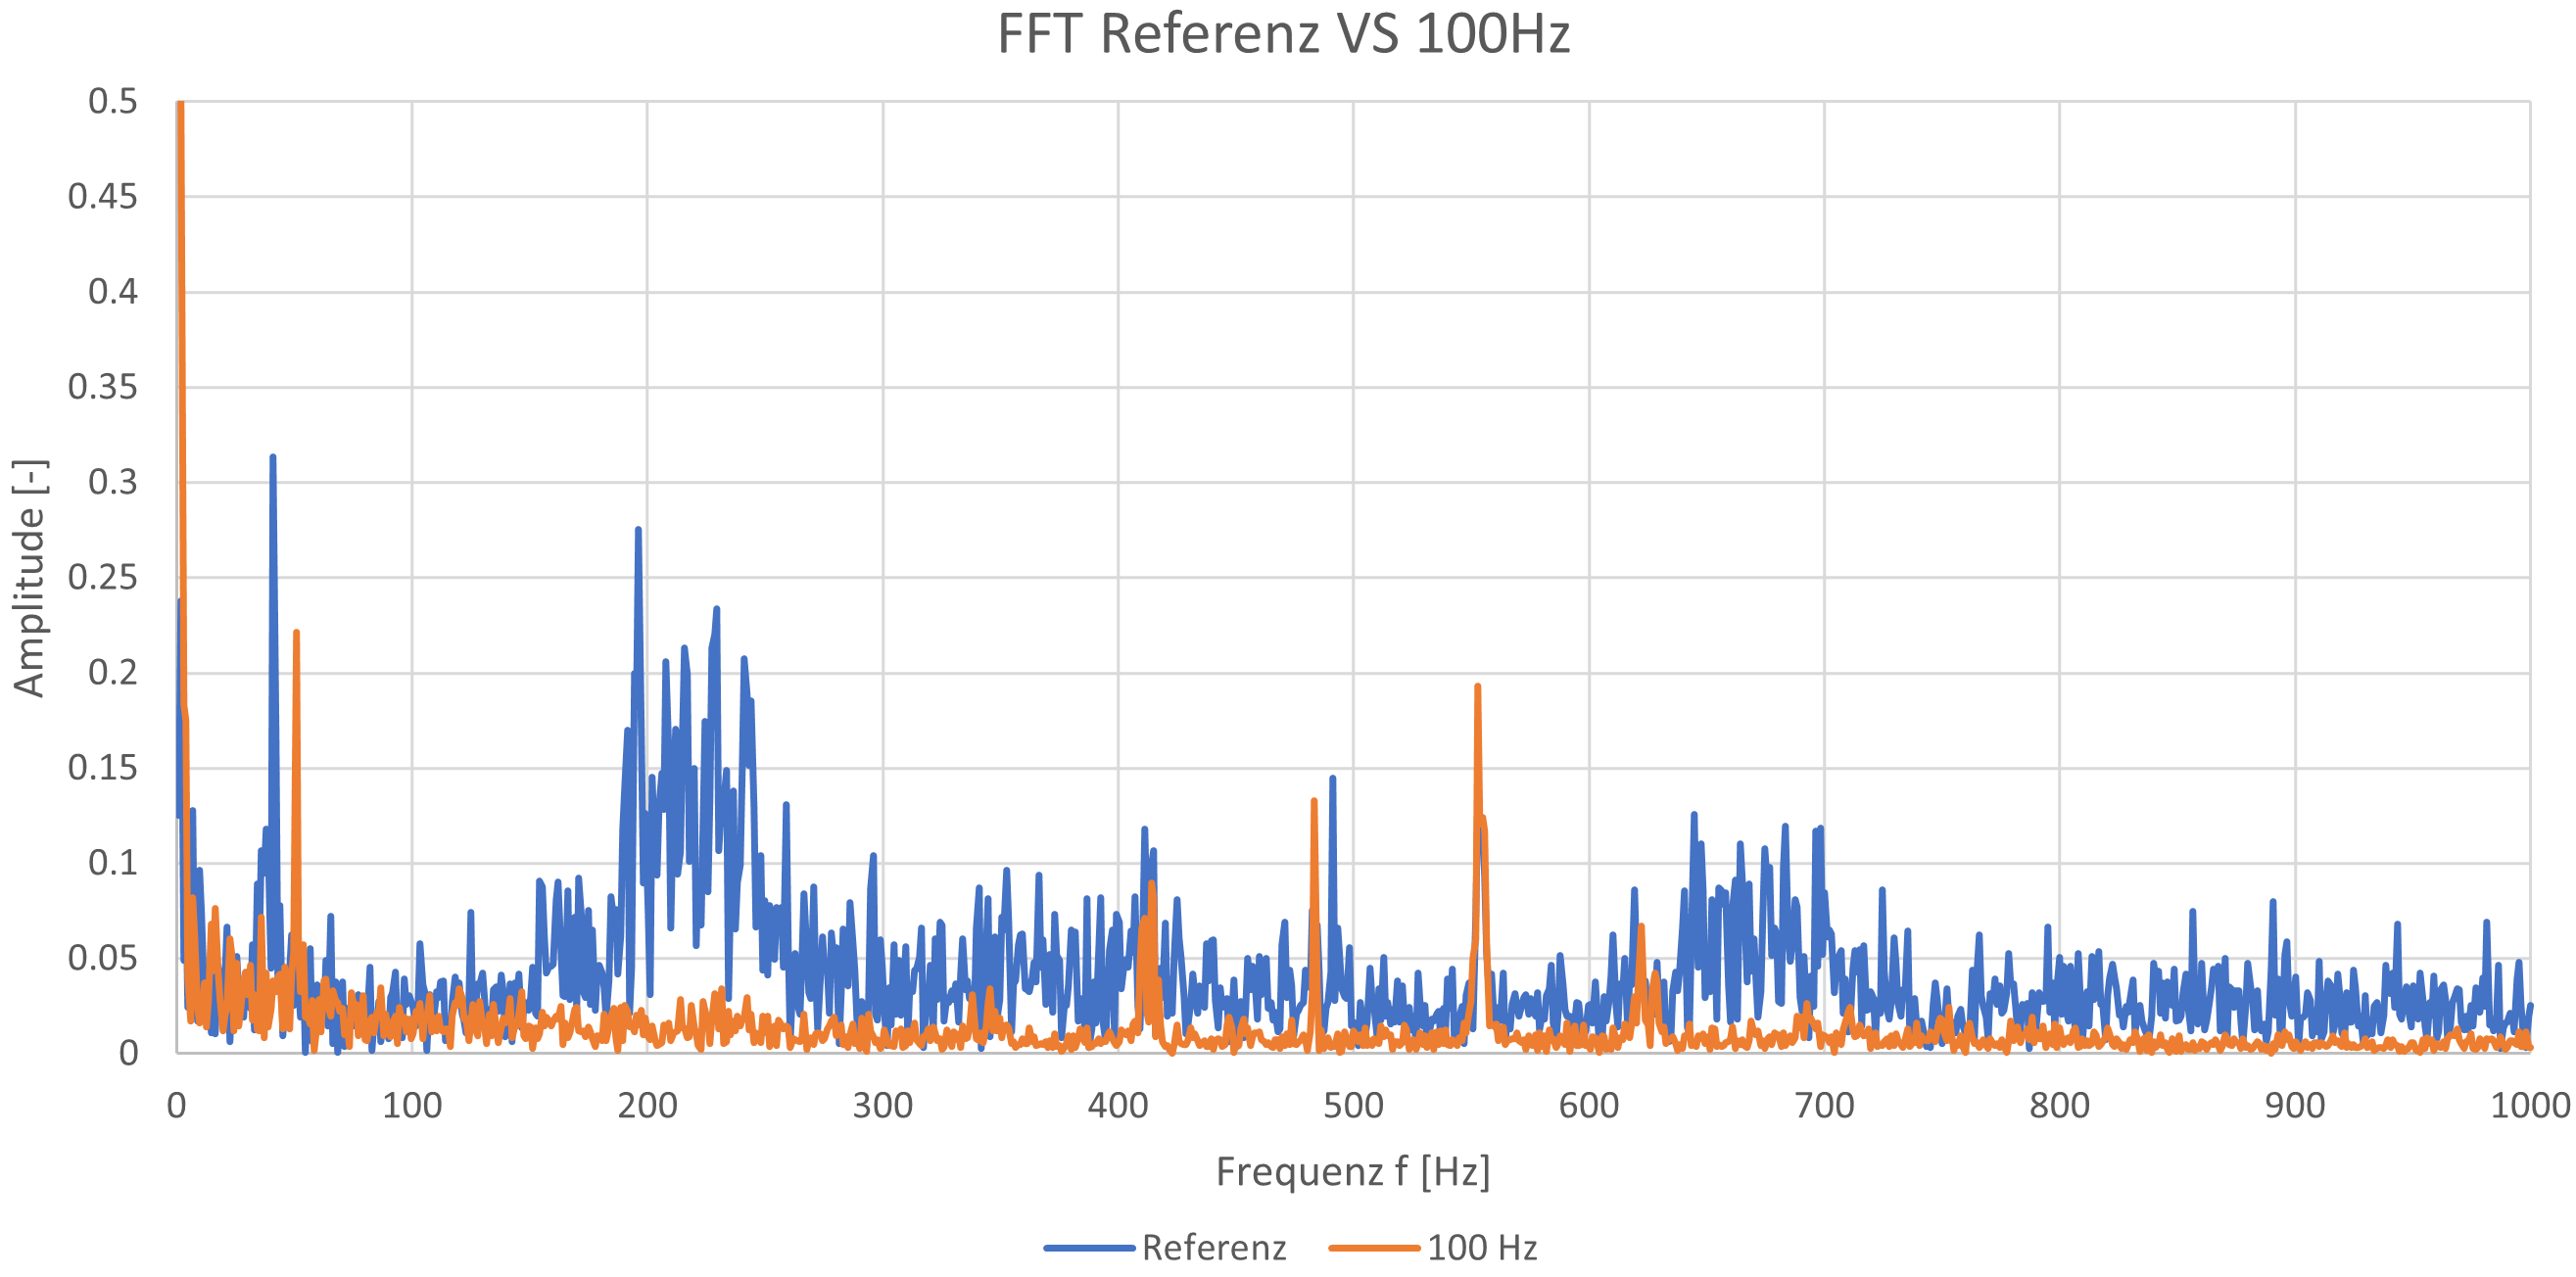
\includegraphics[width=1\linewidth]{FFT100Hz}
		\caption{(Fast) Fouriertransformation der Nullpunktsignale}
		\label{fig:fft100hz}
	\end{figure}	
\noindent Die Messungen für das DuT mit  $f_c=500$Hz wurden nicht in der Tiefe ausgewertet, da der Nullpunkt ähnlich rauscht wie jener der Referenz (im FFT-Diagrammm zu erkennen: Deutliche Amplituden bei 200...300 Hz  $< f_c =500$Hz)
	